\section{Proposta de Implementação de Governança de TI}\label{sec:proposta}

Sabendo que a AEB é um órgão federal que presta serviços a sociedade brasileira, é ideal que o preste com  qualidade e eficiência. Mediante ao cenário exposto na Seção \ref{aeb}, identifica-se que a AEB necessita valorizar a TI para que possa usufruir de grandes benefícios a partir da TI.

Com a implementação da Governança de TI pode-se alcançar resultados concretos e benéficos ao órgão alinhando a TI ao negócio. Mas essa tarefa é complexa e demanda tempo para chegar a resultados satisfatórios, pode-se dizer que é um empreendimento de longo prazo.

 Segundo \cite{ImplantandoGTI:2012}, existem alguns requisitos que devem ser atendidos para sua implantação, como:

\textbf{Liderança para mudança}: instituir um executivo patrocinador que faz parte da alta direção do órgão, para assumir a liderança e garantir os fundos necessários para a implementação.

\textbf{Envolvimento dos executivos da organização}: Envolver os demais executivos do órgão, no caso as diretorias, pois são gestores de processos indispensáveis ao órgão e que podem ser atendidos pela TI.

\textbf{Atacar as principais vunerabilidades}: Deve haver identificação e priorização das principais vulnerabilidades pela Governança de TI, para obter resultados a curto prazo e sucesso do empreendimento. Os resultados obtidos devem ser comparados com anteriores para que as melhorias sejam evidenciadas.

\textbf{Ter uma abordagem de gestão de mudança cultural}: Ao implementar a GTI vão haver várias resistências envolvendo os funcionários da TI, os usuários e os clientes, pois haverão mudanças na execução dos trabalhos. Para isso deverá ser planejada a mudança cultural pela gerência e a presidência, que deverão tomar atitudes condizentes para a implementação.

\textbf{Equipe Qualificada}: Para implementar a GTI deve-se ter pessoas qualificadas e experientes que trabalham com planejamento, implementação e gerencie o processo de implementação.

\textbf{Certificar se os benefícios da implementação de GTI estão sendo atingidos}: A Alta administração só entenderá os esforços que estão sendo investidos se houver retornos visíveis, numéricos e em especial agregar valor ao negócio.


\subsection{Roteiro de Implementação de Governança de TI}

Para implementar está proposta de governança de TI segundo \cite{ImplantandoGTI:2012} é necessário seguir algumas atividades que são de grande importância para obter resultado. A Figura~\ref{fig:roteiro} mostra um roteiro a ser seguido para a implementação da GTI.

\begin{figure}[ht]
\centering
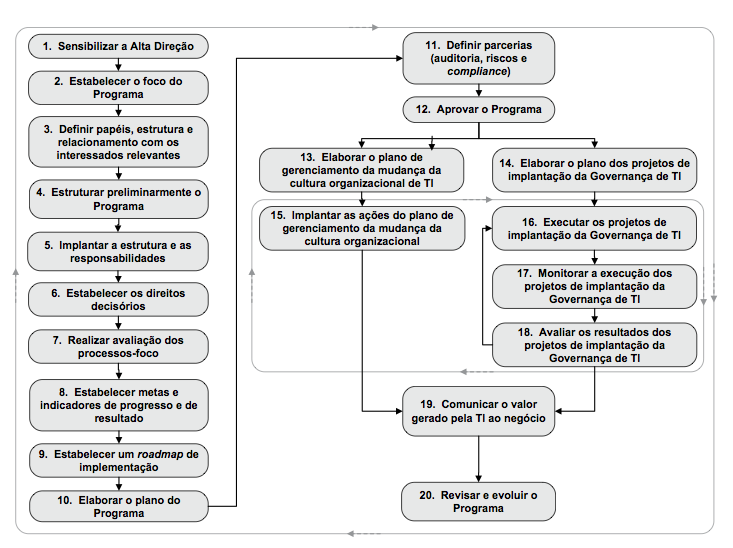
\includegraphics[width=1.0\textwidth]{roteiro.png}
\caption{Proposta de roteiro para implementação de Governança de TI.}
\label{fig:roteiro}
\end{figure}

O roteiro norteia as atividades que deve-se seguir para obter a governança de TI no órgão. Seguiu-se algumas aplicando em dados encontrados no ambiente da AEB. Esse roteiro é complexo e demanda vários ciclos de tarefas para seu êxito. Sugeri-se em algumas delas, atividades que podem ser executadas durante a implementação da GTI, mas em outras foi realizada contextualização da sua importância no processo de implementação da GTI.

\subsubsection{Sensibilizar a Alta Administração}

Sensibilizar a alta direção quanto a importância da TI para o órgão, pois sem seu apoio e patrocínio serão impossíveis. 

A TI na AEB está passando por alguns problemas que podem ser resolvidos com investimentos adequados. Um dos mais importância são os relacionados a segurança dos dados, pois o órgão lida com informações de sigilo como tratados, acordos, dados financeiros, emails organizacional e dados pessoais. Essas informações precisam ser protegidas, em especial nos dias de hoje onde foram evidenciadas espionagens por países vizinhos, apartir de vulnerabilidade ligadas a TI.

Para que a TI esteja alinhada as estratégias do órgão é necessaria a priorização de investimentos em projetos que partiram da tomada de decisão da alta administração.

Os processos de atividades administrativas precisam ser mapeadas e otimizados para que haja uma maior transparência de informações a alto administração.

Com a utilização de metodologias de boas práticas que a TI se baseia, referidas na Seção \ref{sec:govti}, pode-se obter resultados satisfatórios de utilização da TI.

\subsubsection{Objetivos de Implementação da GTI }

Com a aplicação da governança de TI queremos inicialmente identificar os processos e gaps organizacionais para que possa encontrar estratégias em sua otimização.

O Segundo é aplicação de ferramentas que  possibilita o gerenciamento e a transparência do andamento de projetos espaciais.

O terceiro é investir em ferramentas que auxiliam a tomada de decisão dos investimentos espaciais. A partir de informações e critérios atuais e históricos que serão cruzadas para disponibilização em dashboards.

O quarto é mater a continuação do serviço e preocupar-se com a segurança da informação.

\subsubsection{Estrutura da Diretoria de GTI}\label{subsec:estruturaGTI}

A AEB precisa de uma reestruturação na área de TI, foi visto na Seção \ref{sec:TIAEB} que a TI está em um posição abaixo do que costuma acontecer em órgãos federais, no qual a TI é tratada como uma diretoria responsável em agregar valor ao negócio.

Para então se implementar Governança de TI no órgão, deve ser criada uma diretoria responsável pela governança, coordenações e divisões responsáveis pela gerência e execução dos processos.

A Diretoria de Governança de TI será responsável por tomar decisão junto a presidência e as demais diretorias dos investimentos, projetos, contratações e aquisições que poderão ser atendidos pela TI. Analisar os resultados alcançados e identificar oportunidades. Implantar sistemas que atenda os processos do órgão assim como manter o funcionamento, implementar segurança de TI e atender as recomendações do SISP. Assim como fornecer suporte a infraestrutura e o atendimento ao usuário.

A Diretoria será dividida em quatro coordenações:

\textbf{Coordenação de Desenvolvimento} - Será responsável por implementar e manter as aplicações de projetos definidos pela GTI e manter os mecanismos de comunicação internos e externos do órgão, como Site e Intranet.

\textbf{Coordenação de Infraestrutura} - Será responsável por fornecer acesso as aplicações internas e externas através de redes computacionais, a manutenção de equipamentos e suporte ao usuário e a implementação da segurança de informação.

\textbf{Coordenação de Governança de TI} -A coordenação será responsável por mapear os processos, auxiliar na identificação das necessidades do órgão, gerenciar as aplicações, aplicar os modelos de boas práticas de mercado como: CobiT, Itil e PMBOK assim como as recomendações do SISP. E também implementar sistemas e ferramentas que auxiliam a tomada de decisão da alta administração por meio de Business iIntelligence - BI.

\textbf{Coordenação de Gerência de Recursos} - Será responsável por implementar e gerenciar contratos de recursos humanos das empresas que prestam serviço a diretoria, e recursos tecnológicos, assim como sua distribuição e fiscalização.

A Figura~\ref{fig:propostaOrg} contém a estrutura da diretoria proposta:

\begin{figure}[ht]
\centering
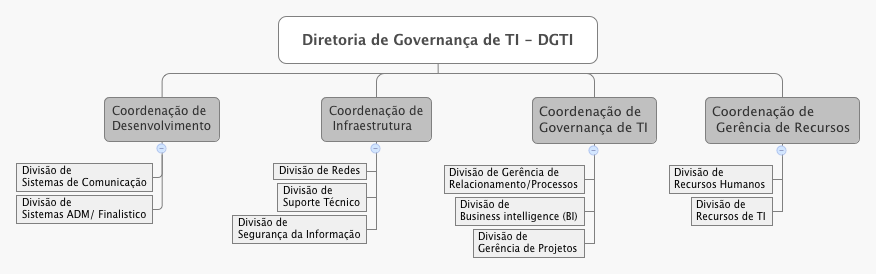
\includegraphics[width=1.0\textwidth]{DGTI.png}
\caption{Proposta de Estrutura Organizacional para GTI}
\label{fig:propostaOrg}
\end{figure}

\subsubsection{Programa de Governança de TI}

Segundo  \cite{ImplantandoGTI:2012}i e o \cite{PMBOK/PMI:2013}, programa é um grupo de projetos gerenciados de forma coordenada a obter benefícios que não estariam disponíveis se os projetos fossem gerenciados individualmente.

Os projetos envolvidos a TI serão gerenciados pela Coordenação de Governança de TI, serão classificados e gerenciados conjuntamente por programas específicos de acordo com o perfil dos projetos. De início sugerimos a criação de dois programas: o responsável por projetos da área meio que auxiliarão a processos administrativos; e os que possuirão projetos voltados a área espaciais que fazem parte da área fim.

\subsubsection{Direitos Decisórios}

O poder de decisão dos investimentos e prioridades serão da Diretoria de Governança de Ti, com participação dos diretores das demais áreas do órgão.  A diretoria de TI estabelecerá como os serviços são cobrados e os resultados desejáveis.

\subsubsection{Avaliação dos Processos}

Para melhorar a avaliação dos serviços prestados e identificar prioridades, foi feito um levantamento das opiniões dos usuários do órgão e chegamos as seguintes prioridades:

\begin{itemize}
\item Projeto de gerência dos recursos humanos, e recursos logísticos, integrado a sistemas fornecido pelo governo.
\item Projeto de gerência de documentos que possibilite uma maior manipulação.
\item Projeto de gerência de equipamento de TI integrado ao de recursos humanos.
\item Melhoria do atendimento ao usuário.
\item Fornecimento de serviços da rede na ausência de energia.
\item Melhoria na segurança das informações.
\end{itemize}

\subsubsection{Estabelecer Metas} \label{subsec:projetos}

Nesta seção, com base no processos identificados, serão definidas as metas.

Projetos ligados a área administrativa como gerência de recursos humanos, almoxarifado e equipamentos de TI, podem ser solucionados com aquisição de Enterprise Resource Planning - ERPs. Para esses projetos a primeira tarefa é estudar a viabilidade de implementação dos ERP. Caso não seja viável será realizada uma estratégia para desenvolvimento da solução no órgão.

O projeto de gerência de documentos já está implementado na casa, mas há a necessidade de incentivar a utilização do sistema na casa. A principal meta é incentivar os gestores a utilizarem e divulgar a solução a seus subordinados. A segunda é identificar as falhas do sistema e tratá-las.
 
A melhoria de atendimento ao usuário é uma atividade constante que não pode ser tratada como um projeto. A meta para essa atividade é implementar um sistema que possibilita a avaliação da TI em suas diversas tarefas, para que a gestão possa elaborar estratégias para melhorar os índices de serviços. 

Para o projeto de fornecimento de serviço da rede na ausência de energia, deverão adotar algumas estratégias. A primeira é aquisição de No Break e geradores para os servidores do prédio sede da rede. Assim com treinar os funcionários para gerênciá-los. 

O projeto de segurança da informação é um dos mais complexos pois além de vários processos envolvidos abrange a cultura organizacional. A primeira meta é mapear e elaborar planos de resposta as vulnerabilidade da TI do órgão. Como segunda seria a implementantação da política de segurança da informação.

\subsubsection{Estabelecer RoadMap de Implantação}

Essa seção trata a sequência, as interdependências, as melhorias e os benefícios a serem alcançados em cada projeto.

No projeto de automação de processos administrativos:

\textbf{Sequência:} Começara pelo levantamento de requisitos, mapeamento dos processos das atividades envolvidas. Logo após pesquisara de uma solução adequada para atender as necessidades e apresentaremos as propostas aos usuários e gestores. Por fim a elaboração do termo de referência para a aquisição da ferramenta e parametrização dos serviços.

\textbf{Interdependências:} O início do projeto depende necessariamente da autorização da governança. Após autorização se inicia o levantamento das necessidades e mapeamento dos processos. Logo após, a aquisição da ferramenta.

\textbf{Melhoria e benefícios:} O projeto otimizará os processos das áreas envolvidas, assim como transparência das informações disponíveis em formulários.

Projeto para gerência de documentos.

\textbf{Sequência:} A gerência de documentos já está implementada, o trabalho é de divulgação da ferramenta. As atividades são de identificar as áreas que utilizarão o sistema e divulgá-lo entre as diretorias. 

\textbf{Interdependências:} Primeiro será feito levantamento das áreas que consumirão o sistema e após isso a divulgação pelas diretorias.

\textbf{Melhoria e benefícios:} Com a divulgação o sistema passará a ser utilizado pelos usuários possibilitando uma maior gerência, pesquisas e substituirão espaços físicos utilizados para a lotação de arquivos.

Melhoria de atendimento ao usuário.

\textbf{Sequência:} A melhoria no atendimento ao usuário conterá as atividades de implementação de sistema de avaliação dos serviços de TI, monitoramento dos serviços resultantes e implementação de boas práticas para o atendimento.

\textbf{Interdependências:} Em primeiro lugar será implementado o sistema de avaliação, logo após serão analisados relatórios das avaliações e em seguida a implementação de boas práticas para sua melhoria. 

\textbf{Melhoria e benefícios:} A atividade contará de três passos que resultarão na otimização dos serviços e na identificação de gargalos.

Projeto de fornecimento de energia:

\textbf{Sequência:} As tarefas da continuidade dos serviços de rede após queda de energia são, aquisição de No Break, sua instalação, aquisição e instalação do gerador de energia para o bloco de lotação da rede e a capacitação dos funcionários para sua gerência. 

\textbf{Interdependências:} O primeiro será a aquisição do No Break. Segundo, a instalação e a aplicação de testes. O terceiro a aquisição do gerador do bloco da rede. Quarto é a capacitação dos funcionários na utilização dos equipamentos.

\textbf{Melhoria e benefícios:} Essas atividades possibilitarão a continuidade dos serviços de rede como sistemas internos, o site e a intranet em quedas de energia.

Implantação da Segurança da Informação:

\textbf{Sequência:} A implementação da Segurança de TI é um projeto complexo pois inicialmente precisa da sensibilização da governança corporativa. As atividades iniciais serão: a concientização da importância do investimento e implementação, levantar e planejar as ações da área e criar a política de segurança da informação.

\textbf{Interdependências:} A primeira atividade é a concientização da governança corporativa, o segundo é o planejamento de ações. O terceiro é a criação da política de segurança de TI.

\textbf{Melhoria e benefícios:} A criação da área  tornarão os serviços de TI mais completos identificando vulnerabilidades, evitando ataques externos, planejando respostas a riscos dentre outros benefícios.

\subsubsection{Plano do Programa de Governança de TI}

O Plano do Programa de Governança de TI conterá um esboço total descrevendo todos os atributos que determinam o sucesso do Programa de Governança.

Segundo \cite{ImplantandoGTI:2012}, são eles:

\begin{itemize}
\item Escopo do programa contendo os processos, estruturas e ações de TI a serem implementados.
\item Sequência de implementação dos processos, respeitando as considerações técnicas requeridas.
\item Linha de tempo prevista para implementação dos processos.
\item O plano de recursos estimados para o programa.
\item Os serviços a serem adquiridos.
\item O orçamento para o programa e para cada um dos projetos. 
\item Os benefícios esperados a serem atingidos, à medida que os processos forem sendo implementados.
\item Plano de gerênciamento do programa.
\item Estrutura de gestão do programa e a matriz de responsabilidades.
\item Riscos do programa.
\item Estratégia de gerência de mudanças.
\item Plano de continuidade do programa.
\item Critérios de qualidades a serem seguidos pelos projetos.
\item Métricas de progresso a serem consideradas pelos projetos componentes do programa.
\item Pontos de controle do programa.
\end{itemize}

Sugere-se que a AEB atente a todos os atributos para que possa ter bons resultados na implementação da Governança de TI e evitando surpresas desagradáveis.

\subsubsection{As Parcerias com Auditoria Interna e Externa}

Segundo o \cite{ImplantandoGTI:2012}, as áreas de auditoria interna e externa são grandes aliadas na implementação de Governança de TI pois têm acesso à Alto Administração. Parceria que se torna importante ao avaliar os processos e identificar as grandes vunerabilidades da TI para o negócio.

Essas informações são muito importantes para o período inicial da governança de TI, mas também durante seu curso. As áreas de auditorias são:

\begin{itemize}	
\item Auditoria Interna.
\item Tribunal de Contas da União - TCU.
\item Controladoria Geral da União - CGU.
\end{itemize}

A área responsável do órgão é a Auditoria Interna que fiscaliza se os processos estão de acordo com requisitos da governança e leis.

O TCU e a CGU se responsabilizam por fiscalizar o órgão como um todo, especialmente na utilização de boas práticas de execução dos projetos, fiscalização de contratos e conformidade com leis que regulamentam os setores.

\subsubsection{Aprovação do Programa}

A aprovação do programa de implementação de GTI, dependerá de autorização da Alto Administração. Na qual ao autorizar a execução do programa, automaticamente autorizará os projetos e recursos financeiros para sua implementação.

\subsubsection{Elaboração do Plano de Mudança da Cultura Organizacional}\label{sec:cultural} 

É necessário entender-se que para o sucesso da implntação da Governança de TI existem pontos chave que precisam ser trabalhados. que são os recursos humanos.

Para haver uma mudança na organização como a criação de uma nova diretoria será necessário elaborar um plano de mudança da cultura organizacional para se alcançar os objetivos desejados. 

Essa atividade demanda uma análise profunda dos processos organizacionais: pessoas, grupos de trabalhos e da estrutura organizacional.

 Portanto não falaremos do plano de mudança, mas sim da sua importância para o sucesso da Implantação da GTI.

A cultura organizacional de acordo com \cite{schein:1985} é:

"Cultura é a experiência que o grupo adquiriu à medida que resolveu seus problemas de adaptação externa e integração interna, e que funciona suficientemente bem para ser considerada válida. Portanto, essa experiência pode ser ensinada aos novos integrantes como forma correta de perceber, pensar e sentir-se em relação a esses problemas".

Ainda de acordo com o autor, para realmente interpretar a cultura de uma organização, deve se ir além dos artefatos visíveis e descobrir os pressupostos básicos fundamentais, que é, como são as relações do centro da cultura da organização. 

Para se aplicar a mudança cultural deve-se:
\begin{enumerate}
\item Avaliar a cultura organizacional atual e definir cultura desejada;
\item Avaliar as gaps entre a cultura atual e deseja;
\item Identificar ações e iniciativas para eliminar os gaps; 
\item Criação de um grupo de gerência de mudança com os líderes de TI da organização;
\item Plano de comunicação, para disseminar o projeto pelo órgão;
\item Programa de capacitação
\item Programa de desenvolvimento de liderança;
\item Estabelecimento de metas;
\item Recursos humanos e orçamentário;
\item Plano de ação com cronograma e responsabilidades.
\end{enumerate}

 A mudança da cultura organizacional é critica para o sucesso do programa.

\subsubsection{Plano dos Projetos}

Essa etapa trás a importância de ter um Plano de Gerenciamento do Projeto para cada um dos projetos especificados anteriormente.

Segundo \cite{PMBOK/PMI:2013}, o Plano de Gerenciamento do Projeto é um documento central que define a base de todo trabalho do projeto. Nele são reunidos todos os planos de gerenciamento auxiliares. O Plano de Gerenciamento de Projeto é definido como o projeto é executado, monitorado, controlado e encerrado.

O plano varia dependendo da área de aplicação do projeto e da complexidade, ou seja, reforça o conceito que cada projeto é singular.

De acordo com \cite{ImplantandoGTI:2012}, o Plano de Gerenciamento de Projeto conterão mas não são limitadas a:

\begin{itemize}
\item Linhas de base do escopo, cronograma e custo;
\item Planos auxiliares resultado de saída de todos os processos do planejamento; 
\item O ciclo de vida selecionado para o projeto e os processos que serão aplicados a cada fase; 
\item Descrição de como o trabalho será executado para alcançar os objetivos do projeto;
\item Um plano de gerenciamento de mudanças que documenta como serão monitoradas e controladas;
\item Requisitos e técnicas para comunicação entre as partes interessadas;
\item Dentre outras.
\end{itemize}

\subsubsection{Implementar Ações do Plano Integrado de Mudanças }

Ao implementar as ações dos projetos referidos na Seção \ref{subsec:projetos}, o Plano de Mudança da Cultura Organizacional deverá estar em execução paralela. 

\subsubsection{Implantar Projetos de GTI}

Para a implementação de GTI foram definidos planos de ações que foram distribuídos em projetos. Esses são os projetos da GTI e são de grande importância para sua implementação. Eles devem ter o mesmo tratamento dos demais quanto a seu ciclo de desenvolvimento e respeitando os processos dos grupos planejamento, execução, monitoramento e controle, e o encerramento.

\subsubsection{Monitorar Projetos de Implantação de GTI}

Os projetos da implementação deverão ser monitorados para avaliar e identificar seu andamento, a qualidade dos entregáveis, a gerência do escopo, gerência de risco e respostas, gerência de cronograma, e gerência do tempo.

\subsubsection{Avaliação dos Resultados} 

Após as entregas dos projetos é necessário identificar se os resultados foram alcançados.

Essa avaliação contribuirá para a melhoria dos processos de gerência de projetos, pois saberá se estão havendo boas práticas na fase de planejamento durante a implementação.
 
\subsubsection{Comunicar o Valor Gerado da TI ao Negócio}
 
 Após a implementação da Governança de TI os resultados de projetos devem ser entregues a governança corporativa, ou seja, as diretorias. 
 
 Os resultados esperados são aqueles desenvolvidos de acordo com o requerido e entregue no prazo. Outro é ser capaz de atender a expansão do negócio rapidamente e resolução rápida dos incidentes, também as inovações tecnológicas e plataformas flexíveis para acompanhar o crescimento do negócio.
 
 Todos os projetos deverão ser identificados quais os requisitos de sucesso do negócio serão atingidos.
 
 \subsubsection{Revisar e Evoluir o Programa de Governança de TI}
 
 Assim que os projetos forem entregues se espera que a cultura organizacional evolua. Pois índices de melhorias se tornarão visíveis.
 
 No entanto, o programa não para por ai, projetos de melhoria deverão ser identificados e planejados, assim como novos projetos e oportunidades. 
 
 A mudança no foco estratégico deverá ser identificada pois também ocasiona a evolução do programa de Governança de TI, que imediatamente deve ser planejada recomeçando novamente o ciclo.
 
